%  article.tex (Version 3.3, released 19 January 2008)
%  Article to demonstrate format for SPIE Proceedings
%  Special instructions are included in this file after the
%  symbol %>>>>
%  Numerous commands are commented out, but included to show how
%  to effect various options, e.g., to print page numbers, etc.
%  This LaTeX source file is composed for LaTeX2e.

%  The following commands have been added in the SPIE class 
%  file (spie.cls) and will not be understood in other classes:
%  \supit{}, \authorinfo{}, \skiplinehalf, \keywords{}
%  The bibliography style file is called spiebib.bst, 
%  which replaces the standard style unstr.bst.  

\documentclass[]{spie}  %>>> use for US letter paper
%%\documentclass[a4paper]{spie}  %>>> use this instead for A4 paper
%%\documentclass[nocompress]{spie}  %>>> to avoid compression of citations
%% \addtolength{\voffset}{9mm}   %>>> moves text field down
%% \renewcommand{\baselinestretch}{1.65}   %>>> 1.65 for double spacing, 1.25 for 1.5 spacing 
%  The following command loads a graphics package to include images 
%  in the document. It may be necessary to specify a DVI driver option,
%  e.g., [dvips], but that may be inappropriate for some LaTeX 
%  installations. 
\usepackage[]{graphicx}

\title{Texture mapping 3D planar models of indoor environments with noisy camera poses} 

%>>>> The author is responsible for formatting the 
%  author list and their institutions.  Use  \skiplinehalf 
%  to separate author list from addresses and between each address.
%  The correspondence between each author and his/her address
%  can be indicated with a superscript in italics, 
%  which is easily obtained with \supit{}.

\author{Peter Cheng, Michael Anderson, Stewart He, Avideh Zakhor
\skiplinehalf
University of California, Berkeley\\
}

 

%%%%%%%%%%%%%%%%%%%%%%%%%%%%%%%%%%%%%%%%%%%%%%%%%%%%%%%%%%%%% 
%>>>> uncomment following for page numbers
% \pagestyle{plain}    
%>>>> uncomment following to start page numbering at 301 
%\setcounter{page}{301} 
 
\begin{document}
\maketitle

%%%%%%%%%%%%%%%%%%%%%%%%%%%%%%%%%%%%%%%%%%%%%%%%%%%%%%%%%%%%% 
\begin{abstract}
  Automated 3D modeling of building interiors is used in applications
  such as virtual reality and environment mapping. Texturing these
  models allows for photorealistic visualizations of the data
  collected by such modeling systems. Camera poses obtained by these
  systems often suffer from inaccuracies, resulting in visible
  discontinuities when successive images are projected adjacently onto
  a surface for texturing. Existing methods to stitch images together
  are often computationally expensive and work independently of pose
  estimates and geometry information. We propose a method to refine
  camera poses using both existing estimates and geometry information,
  followed by two different methods to composite images together,
  based on the uniformity of available images. The effectiveness of
  our methods is demonstrated on a number of different indoor
  environments.
\end{abstract}

% >>>> Include a list of keywords after the abstract

\keywords{Texture Mapping, Reconstruction, Image Stitching, Mosaicing}

%%%%%%%%%%%%%%%%%%%%%%%%%%%%%%%%%%%%%%%%%%%%%%%%%%%%%%%%%%%%%
\section{INTRODUCTION}
\label{sec:introduction} % \label{} allows reference to this section
Three-dimensional modeling of indoor environments has a variety of
applications such as training and simulation for disaster management,
virtual heritage conservation, and mapping of hazardous sites. Manual
construction of these digital models can be time-consuming, and as a
result, automated 3D site modeling has garnered much interest in
recent years. CITATION

The first step in automated 3D modeling is the physical scanning of
an environment's geometry. An indoor modeling system must recover its
own poses within an environment while simultaneously reconstructing
the 3D structure of the environment itself. CITATION. This is known as
the simultaneous localization and mapping (SLAM) problem, and is
generally solved by taking readings from laser range scanners,
cameras, and inertial measurement units (IMUs) at multiple locations
within the environment.

In this paper, we work with data obtained from a backpack-mounted
system, carried by an ambulatory human. Such a system provides
advantages over more common wheel-mounted systems in terms of agility
and portability, but results in much higher localization error and
uncertainty overall. CITATION. As a result, common methods for texture
mapping generally produce poor results, leading to the development of
the approaches contained in this paper. Besides localization
information and images, environment geometry is required as well for
texture mapping. In this paper we work mainly with models obtained
by fitting planar surfaces to point clouds generated by the
backpack system. CITATION. We have also developed an appropriate
method to work with near-planar triangular meshes, as described in APPENDIX
SOMETHING.

Though our texture mapping procedure was designed with the
aforementioned system in mind, it is easily generalizable to any other
system, provided the required inputs of planar geometry, images with
rough extrinsic pose estimates, and either known or estimated
intrinsic camera calibration matrices. An important benefit of our method
is its relatively low complexity and modularity of each step,
allowing for quick tuning of parameters and easy accomodation of new
input data given updates in localization or model-generation
algorithms.

The remainder of the paper is organized as follows. Section X explains
how input images are projected onto our geometry and simple approaches
towards texturing. Section X covers more sophisticated existing
approaches to image matching and stitching, and their performance on
our datasets. Section X contains our approach towards image alignment,
followed by Section X, which describes compositing approaches. Section
X contains further results and conclusions.
%%%%%%%%%%%%%%%%%%%%%%%%%%%%%%%%%%%%%%%%%%%%%%%%%%%%%%%%%%%%%

\section{Simple Texture Mapping}
\label{sec:simpleTextureMapping}
\begin{figure}
  \centering
  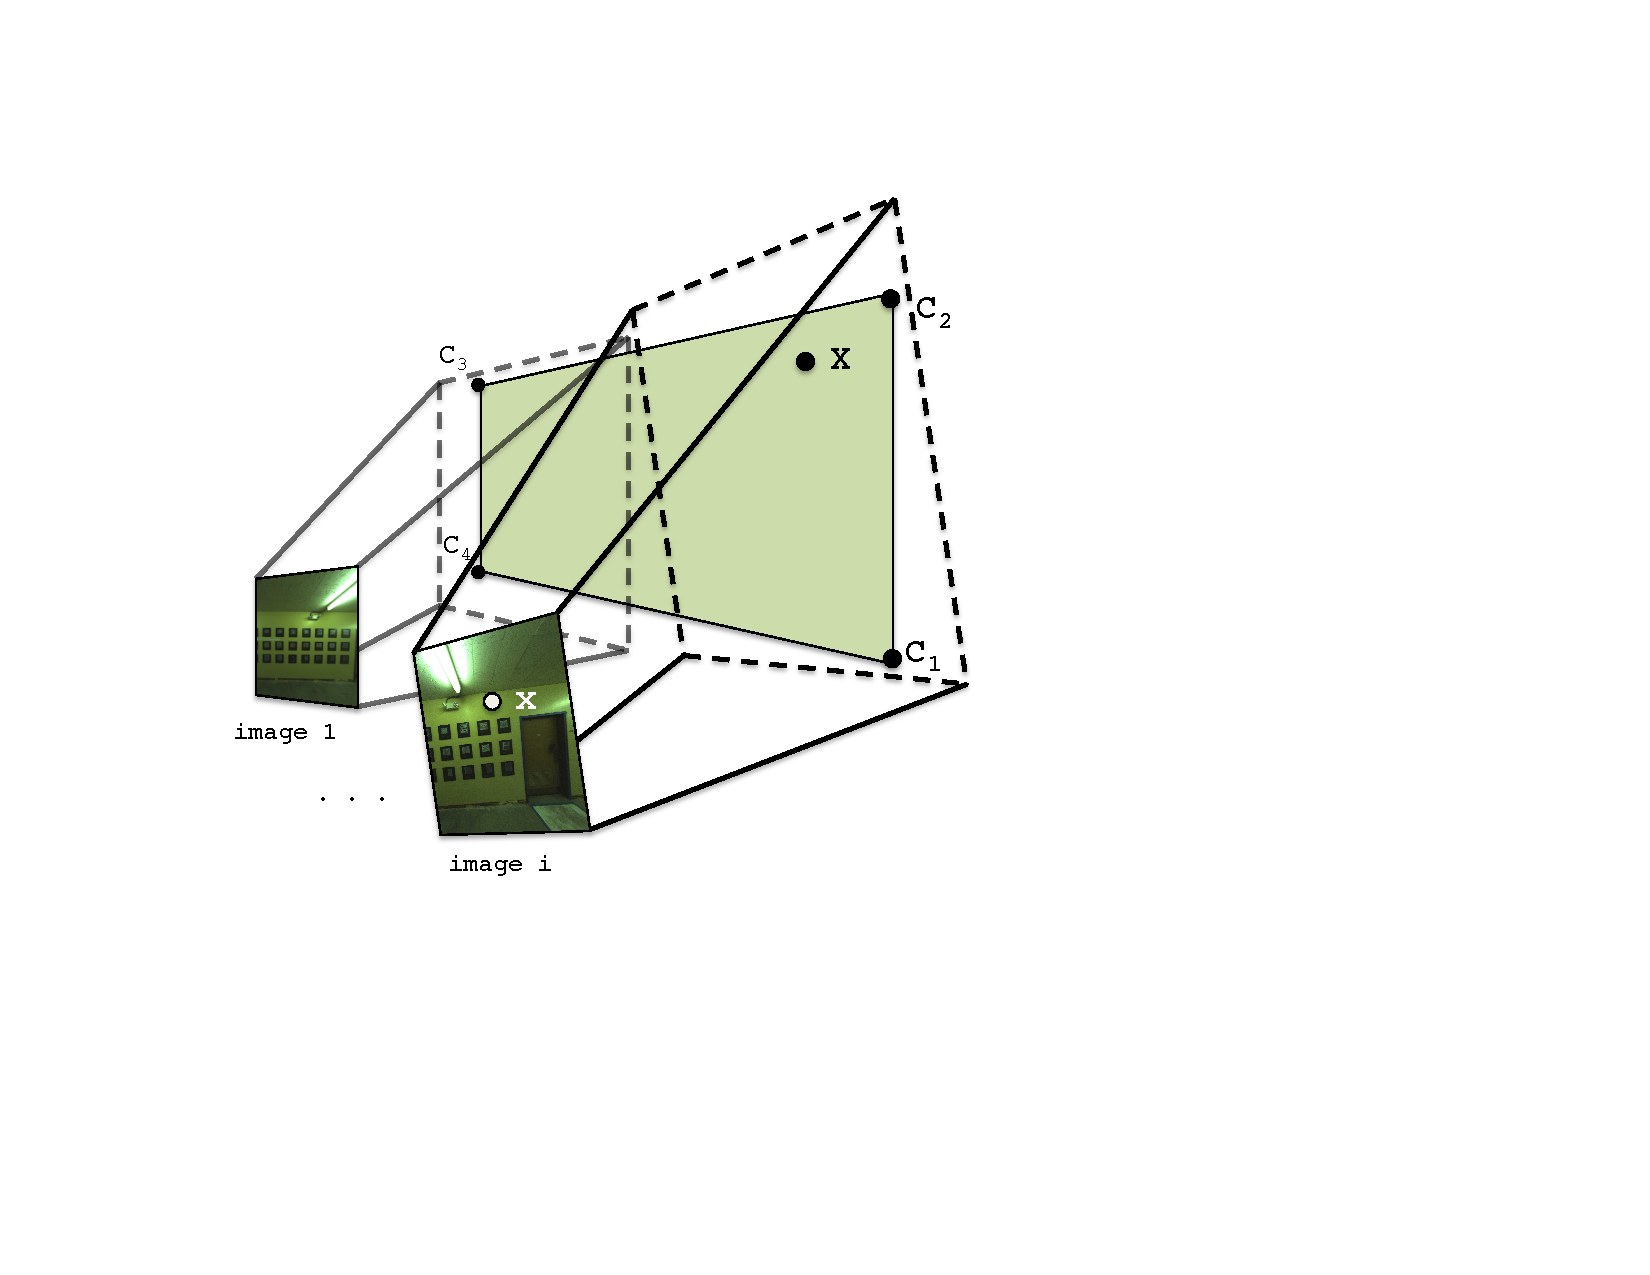
\includegraphics[height=2in]{Projection.pdf}
  \caption{Planes are specified in 3D space by four corners $C_1$ to
    $C_4$. Images are related to each plane through the camera matrics
    $P_{1..m}$. }
  \label{fig:projection}
\end{figure}

The geometry of the texture mapping process for a plane is shown in
Figure \ref{fig:projection}.  As described earlier, we are provided
with a set of $M$ images to texture the target plane. Each image has a
camera matrix $P_i$ for $i=1..M$, which translates a 3D point in the
world coordinate system to a 2D point or pixel in image $i$'s
coordinates. A camera matrix $P_i$ is composed of the camera's
intrinsic parameters, such as focal length and image center, as well
as extrinsic parameters which specify the rotation and translation of
the camera's position in 3D world coordinates at the time that image
$i$ is taken. These extrinsic parameters are determined by the
backpack hardware and localization algorithms \cite{chen2010indoor,
  liu2010indoor, kua2012loopclosure} and are quite noisy.

Because our backpack system takes photos at a rate of 5 Hz, thousands
of images are available for texturing each surface in our model. Our
goal in designing a texture mapping process is to decide which of
these images should be used, and where their contents should map onto
the texture, in order to minimize any visual discontinuities or seams
that would suggest that the plane's final texture is not composed of a
single continuous image.

Ignoring the fact that the camera matrices $P_{1..M}$ are inaccurate,
we can texture the plane by discretizing it into small square tiles,
in our case 5 pixels across, and choosing an image to texture each
tile.

We choose to work with rectangular units to ensure that borders
between any two distinct images in the final texture are either
horizontal or vertical. Since most strong environmental features
inside buildings are horizontal or vertical, any visible seams in our
texture intersect them minimally and are less noticeable.

In order to select an image for texturing a tile $t$, we must first
gather a list of candidate images that contain all four of its
corners, which we can quickly check by projecting $t$ into each image
using the $P_i$ camera matrices. Furthermore, each candidate image
must have been taken at a time when its camera had a clear
line-of-sight to $t$, which can be calculated using standard
ray-polygon intersection tests between the camera location, $t$, and
every other plane \cite{rayintersection}.

Once we have a list of candidate images for $t$, we define a scoring
function in order to objectively select the best image for texturing
$t$. Since camera pose errors compound over distance, we wish to
minimize the distance between cameras and the surfaces they
texture. Additionally, we desire images that are projected
perpendicularly onto the plane, maximizing the resolution and amount
of useful texture available in their projections, as well as
minimizing any parallax effects due to real-world geometry not
accurately represented by our digital model. In other words, we wish
to minimize the angle between the tile's normal vector and the camera
axis for images selected for texture mapping. These two criteria can
be met by maximizing the function $\frac{1}{d} (-1 \cdot \vec{c})
\cdot \vec{n}$ as shown in Figure
\ref{fig:scoringFunction}. Specifically, $d$ is the distance between
the centers of a camera and a tile, and $\vec{n}$ and $\vec{c}$ are
the directions of the plane's normal and the camera axis respectively.

\begin{figure}
  \centering
  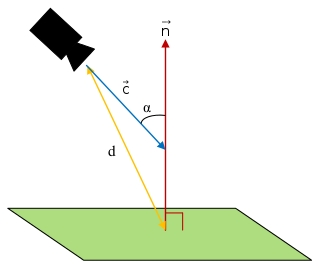
\includegraphics[height=1.5in]{scoringFunction.jpg}
  \caption{We minimize camera angle $\alpha$ and distance $d$ by
    maximizing the scoring function $\frac{1}{d} (-1 \cdot \vec{c})
    \cdot \vec{n}$}
  \label{fig:scoringFunction}
\end{figure}



\begin{figure}[h!]
  \centering \subfloat[][]{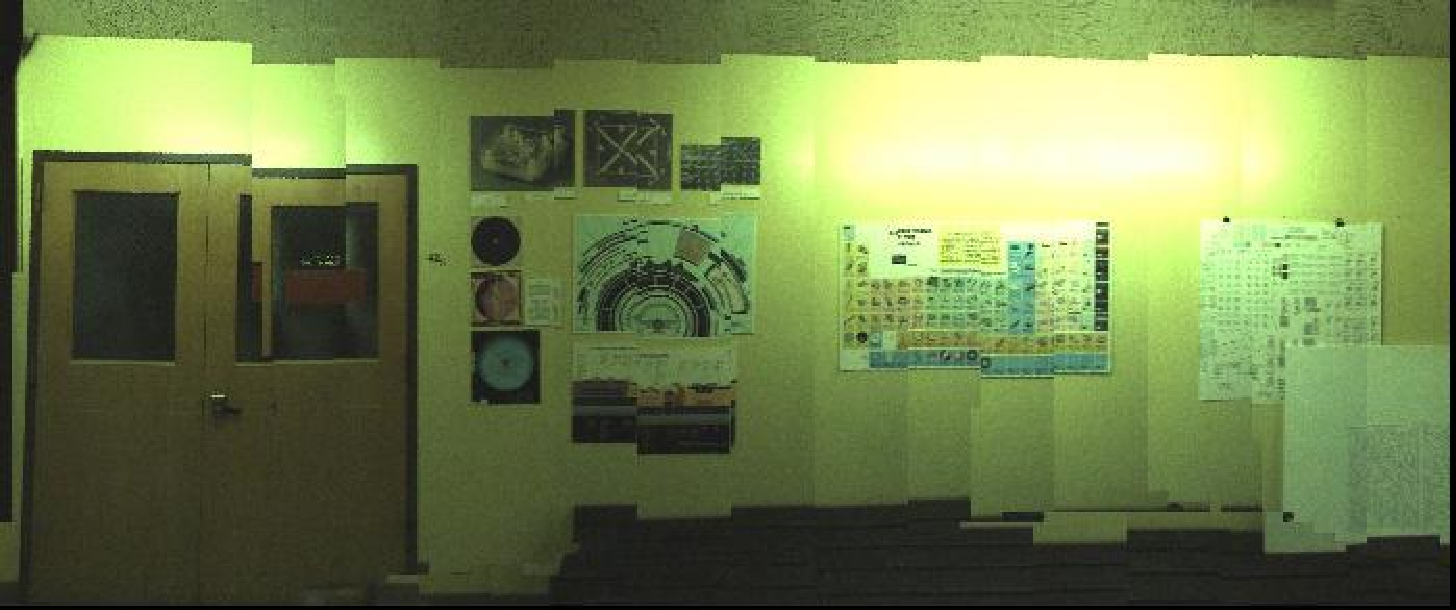
\includegraphics[width=3in,
    height=0.97in]{wall2_naive.pdf}}

  \centering \subfloat[][]{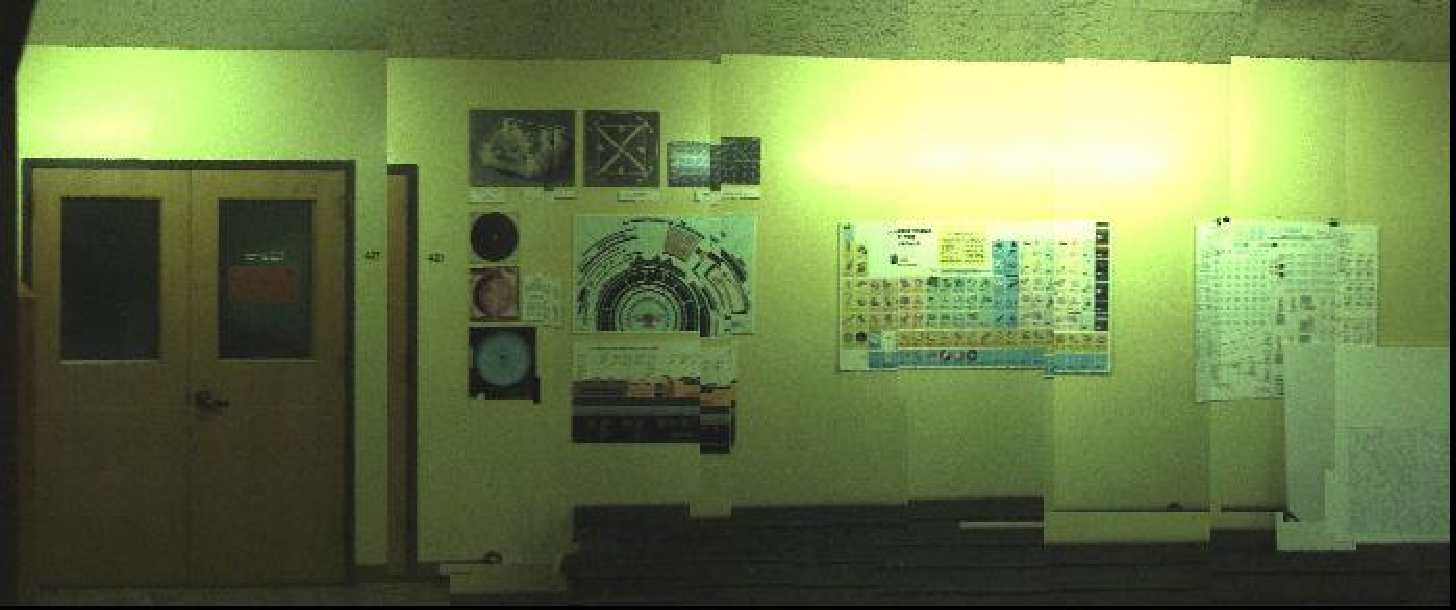
\includegraphics[width=3in,
    height=0.97in]{wall2_cache.pdf}}

  \centering \subfloat[][]{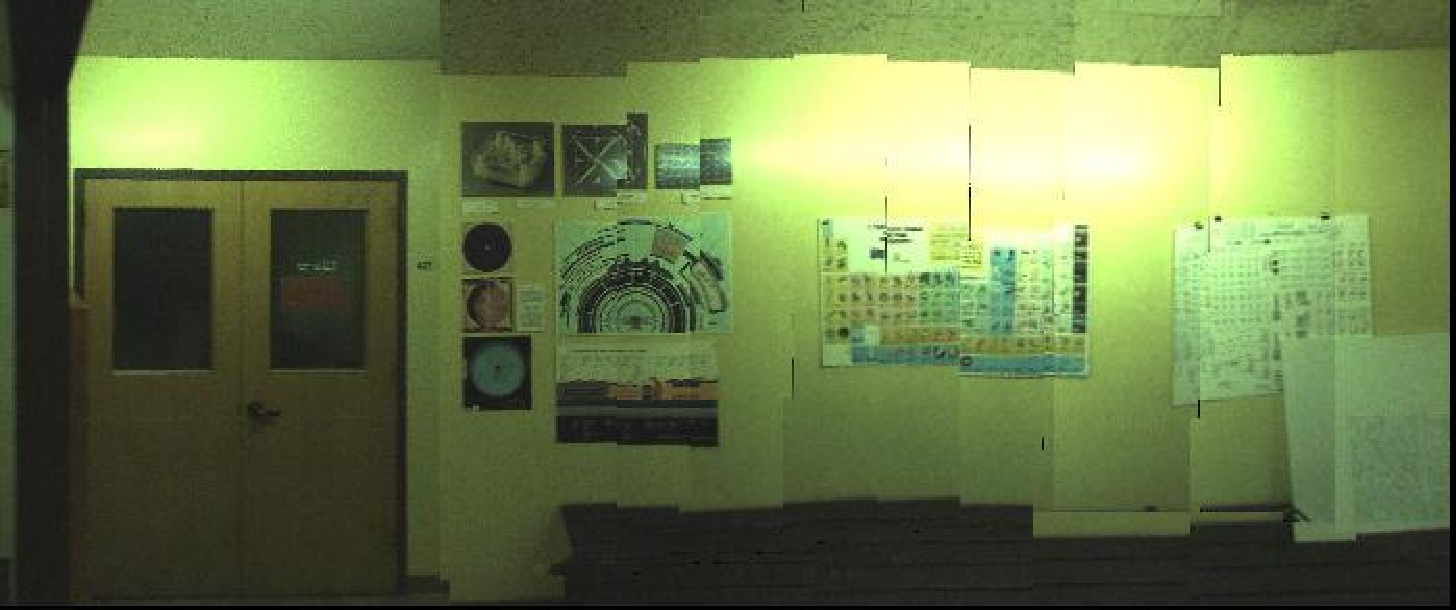
\includegraphics[width=3in,
    height=0.97in]{wall2_cache_shift.pdf}}

  \centering \subfloat[][]{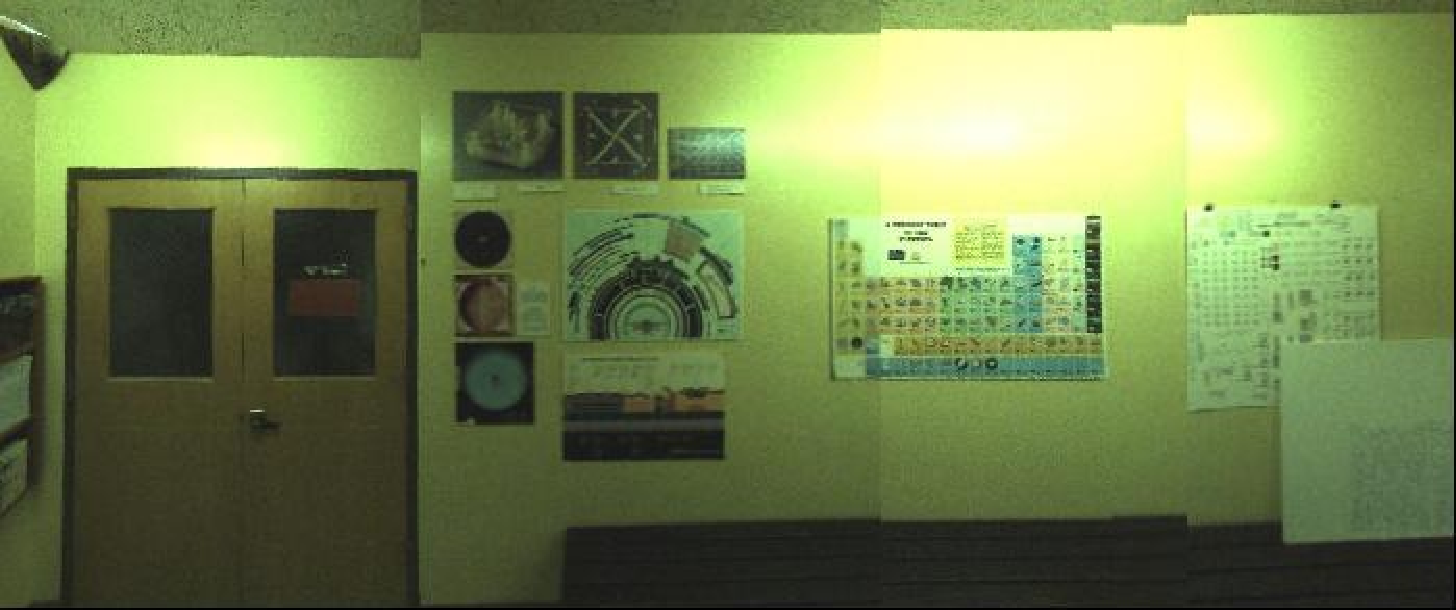
\includegraphics[width=3in,
    height=0.97in]{wall2_dynprog_noblend.pdf}}

  \centering \subfloat[][]{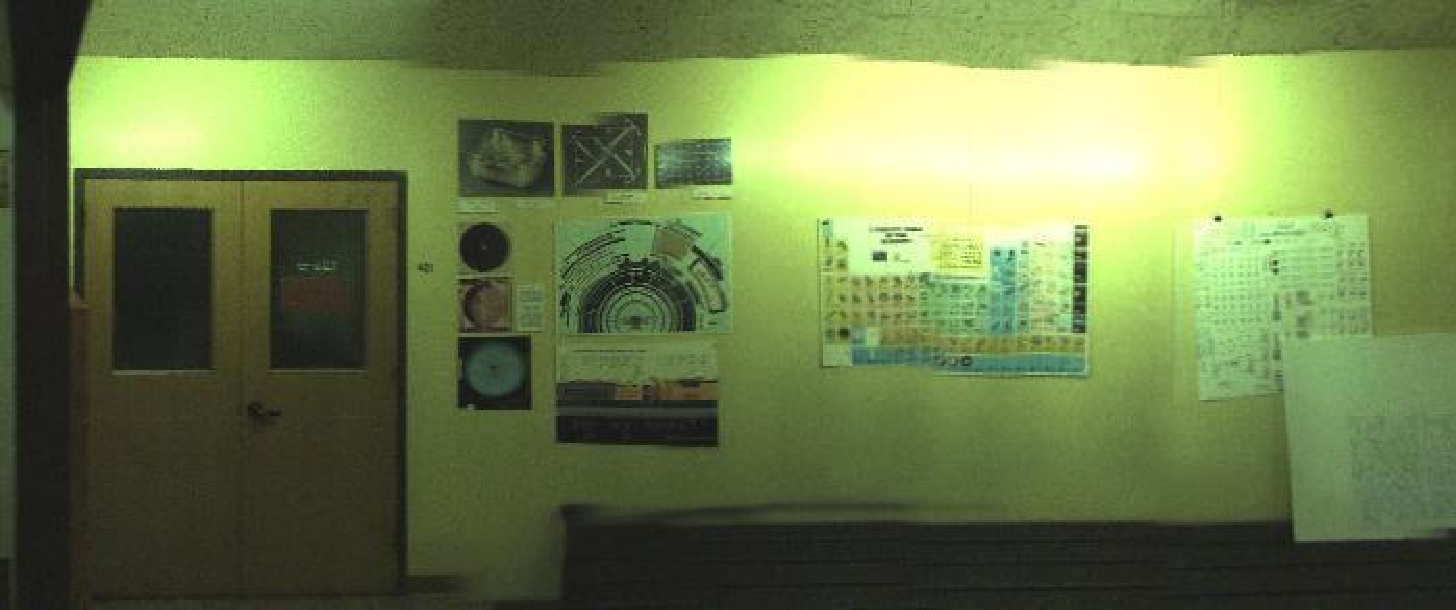
\includegraphics[width=3in,
    height=0.97in]{wall2_cache_shift_blend.pdf}}

  \centering \subfloat[][]{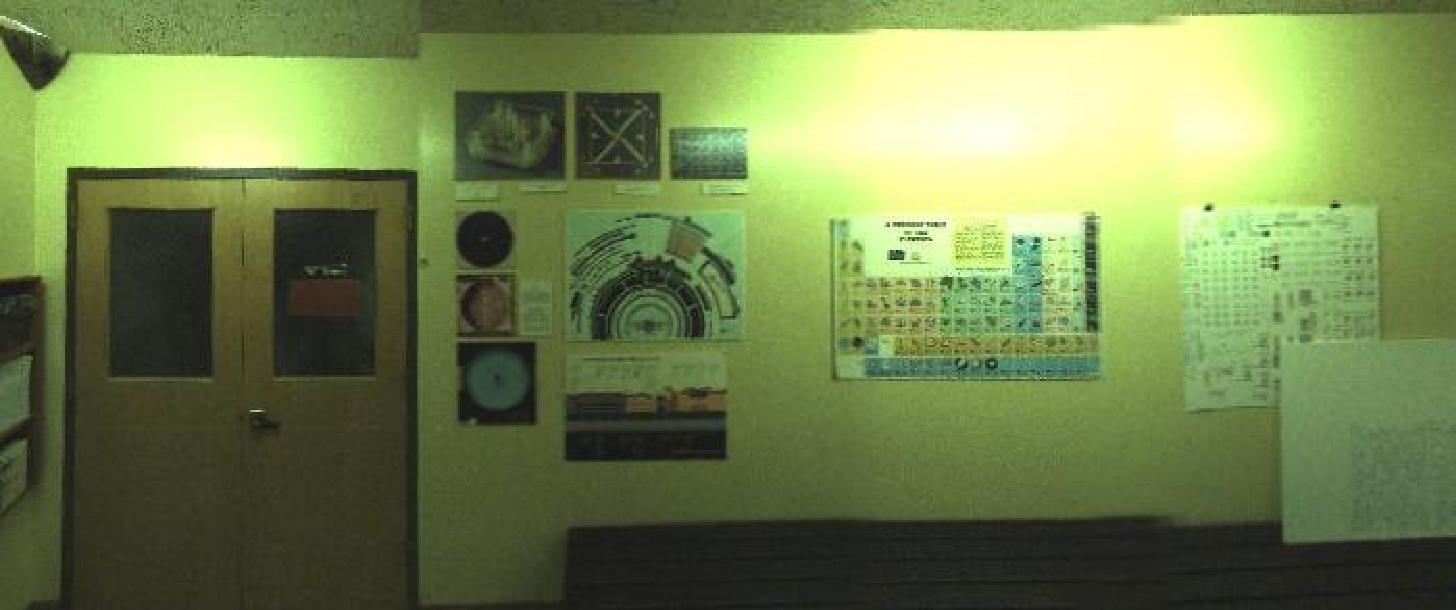
\includegraphics[width=3in,
    height=0.97in]{wall2_dynprog.pdf}}
  \caption{(a) Direct mapping. (b) Mapping with caching. (c) Mapping
    with caching after image alignment. (d) Seam minimization after
    image alignment). (e) same as (c) with blending. (f) same as (d)
    with blending.}
  \label{fig:compareAll}
\end{figure}


As Figure \ref{fig:compareAll}(a) demonstrates, this approach leads to
the best texture for each tile independently, but overall results in
many image boundaries with abrupt discontinuities, due to significant
misalignment between images. Given our high number of input images, one approach might be to more intelligently only select images that match up well, but the far more robust solution is to match up images directly such that we maximize our amount of useful images.



\section{Existing Approaches to Image Alignment}
\label{sec:existingApproaches}
Stitching together multiple images to produce a larger image is a
commonly performed task, with many successful approaches over the past
few decades. Parts of images are first matched to eachother, through
direct pixel comparisons, or more commonly through feature detection
and matching. Images are then adjusted to maximize matches, either by
directly calculating homographies between pairs of images, or by
modifying camera poses from 1 to 6 degrees of freedom.

Feature detection and matching works best when multiple unique visual
references exist in the environment and are present within multiple
images. This allows for accurate matching when texturing detailed
objects at high resolutions CiTATION, or when creating outdoor
panoramas CITATION. In contrast, our indoor environments have a high
prevalence of bare surfaces, as well as repeating textures that cause
difficulty in distinguishing features. The lack of strong reference
points results in high uncertainty when matching images together.

Additionally, our datasets often contain long chains of images, which
leads to error accumulation when image correspondences are not
accurate. For example, when matching a long chain of images through
homographies, a pixel in the $nth$ image must be translated into the
first image's coordinates by multiplying by the $3\times3$ matrix $H_1
H_2 H_3 ... H_n$. Any error in one of these homography matrices is
propagated to all further images, resulting in drift. Figure
\ref{fig:mosaic3D}(b) shows the output of the AutoStitch software
package, which performs homography-based image mosaicing
\cite{autostitch}. Even with many features spread across this surface,
the mosaicing produces errors that cause straight lines to appear as
distorted, despite the fact that it was generated after careful hand
tuning. Many areas with fewer visual features simply failed outright
using this approach.

\begin{figure}
  \centering
  \subfloat[][]{
\includegraphics[width=3in]{Graph_crop.pdf}}

  \centering \subfloat[][]{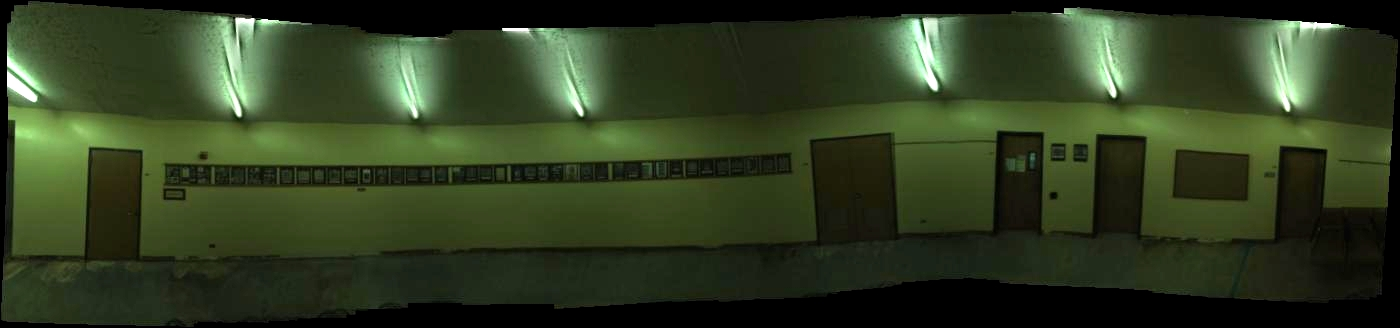
\includegraphics[width=3in]{panoMy.jpg}}
  \caption{Texture alignment via (a) the graph-based localization
    refinement algorithm from \cite{chen2010indoor} and (b) image
    mosaicing.}
  \label{fig:mosaic3D}
\end{figure}

Image projections can also be aligned by iteratively adjusting camera
poses to maximize matches. This is generally done over 6 degrees of
freedom. CITATION. Applying the approach in the LIU2010INDOOR paper
however, results again in error accumulation and drift as shown in
Figure \ref{fig:mosaic3D}(a). Furthermore, such nonlinear optimization
approaches have an extremely high complexity and runtime, and the
entire solution must be recomputed given any changes in input data.


\section{Efficient Image Alignment with Geometry Information}

In this section, we describe our method of efficient and robust image
alignment. Our approach consists of four parts. First, all images are
projected onto the surface and rotated such that detected lines within
them are parallel to lines comprising the surface's boundary and
intersection with other surfaces. Next, these projections are shifted
such that interior lines near surface intersections are matched
up. Following this, occlusion checks are performed across each image
to remove invalid parts of each image for the target surface. These
first three steps are all image-independent and can be considered
pre-processing steps and performed in parallel. Finally, we detect
SIFT feature matches between pairs of images and solve a linear least
squares problem in 2D to maximize matches.

\subsection{Geometry-based Alignment}
\label{sec:projectionAndRotation}
After computing each image's projection onto the target surface, as
described in Section \ref{sec:simpleTextureMapping}, we can detect
lines in the projections using Hough transforms. Experience and
intuition show that walls in indoor environments contain linear
features that are either horizontal or vertical, often corresponding
to doors, windows, posters, etc. Thus, when texturing walls, we rotate
images in 2D such that dominant lines are made to be horizontal or
vertical. Though not as relevant in our datasets, this can be extended
such that lines are oriented with a wall's boundaries, for example in
areas with a slanted roof.

At this point in time, image occlusions have not been accounted
for. As a result, some image projections contain texture that should
project to an adjacent surface, generally with a linear boundary where
the two surfaces meet. If this linear boundary is detected by Hough
transform, it makes sense to rotate and align this boundary such that
the visual boundary between two surfaces matches the physical boundary
in our digital model.

To perform the rotation and alignment, we do MAGIC.  Then we indicate
that magic has been done so that in the next step stuff is good. Mark
as anchor images.

\subsection{Image Occlusion}
get from github i guess i dunno. or check avz email

\subsection{2D Feature Alignment}
\label{sec:robustSIFTFeatureMatching}
Our next step is to align overlapping images by searching for
corresponding points between all pairs of overlapping images. We use
SIFT features for their high detection rate, and choose to use feature
alignment rather than intensity-based alignment due to the differences
in lighting as well as possible occlusion among our images, both of
which feature alignment is less sensitive to \cite{lai1999robust,
  lowe1999object, mikolajczyk2005performance, szeliski2006image}.
SIFTGPU MORE CITATION SIFT matches determine $d^x$ and $d^y$ distances
between each pair of features for two images on the plane, though
these distances may not always be the same for different
features. Since indoor environments often contain repetitive features
such as floor tiles or doors, we need to ensure that SIFT-based
distances are reliable. In order to mitigate the effect of incorrect
matches and outliers, the RANSAC framework \cite{fischler1981random}
is used for a robust estimate of the optimal $d^x_{i,j}$ and
$d^y_{i,j}$ distances between two images $i$ and $j$. The RANSAC
framework handles the consensus-building machinery, and requires a
fitting function and a distance function. For this application, the
fitting function simply finds the average distance between matches in
a pair of images. The distance function for a pair of points is chosen
to be the difference between those points' SIFT match distance and the
average distance computed by the fitting function. We use a 10 pixel
outlier threshold, so that SIFT matches are labeled as outliers if
their horizontal or vertical distances are not within 10 pixels of the
average distance computed by the fitting function.

We now use the $d^x_{i,j}$ and $d^y_{i,j}$ distances between each pair
of images to refine their positions using least squares. Recall that
there are a total of $M^{2}$ possible pairs of images, though we only
generate distances between images that overlap at SIFT feature
points. Given these distances and the original image location
estimates, we can solve a least squares problem
($\textrm{min}_{\vec{\beta}} ||A \vec{\beta} - \vec{\gamma}||_2^2 $)
to estimate the location of the images on the plane. The
$M$-dimensional vector $\vec{\beta}$ represents the unknown $x$
location of each image on the plane for $1 \dots M$. The optimal $x$
and $y$ locations are obtained in the same way, so we only consider
the $x$ locations here:

\[\vec{\beta} =
\begin{pmatrix}
  x_1, & x_2, & x_3, & \cdots & x_{M-1}, & x_M
\end{pmatrix}
\]

The $N \times (M+1)$ dimensional matrix $A$ is constructed with one
row for each pair of images with measured distances produced by the
SIFT matching stage. A row in the matrix has a $-1$ and $1$ in the
columns corresponding to the two images in the pair. For example, the
matrix below indicates a SIFT-based distance between images 1 and 2,
images 1 and 3, images 2 and 3, etc.
\[
A =
\begin{pmatrix}
  -1 & 1 & 0 & \cdots & 0 & 0\\
  -1 & 0 & 1 & \cdots & 0 & 0\\
  0 & -1 & 1 & \cdots & 0 & 0\\
  \vdots  & \vdots & \vdots & \ddots & \vdots  & \vdots\\
  0 & 0 & 0 & \cdots & 1 & 0 \\
  0 & 0 & 0 & \cdots & -1 & 1 \\
  1 & 0 & 0 & \cdots & 0 & 0 \\
\end{pmatrix}
\]
If only relative distances between images are included then there is
no way to determine the absolute location of any of the images and the
matrix becomes rank deficient. To fix this we choose the first image
to serve as the anchor for the rest, meaning all the absolute
distances are based on its original location. This is done by adding a
row with a $1$ in the first column and the rest zeros.

Finally, the $N$-dimensional observation vector $\vec{\gamma}$ is
constructed using the SIFT-based distances generated earlier in the
RANSAC matching stage. The last element in the observation vector is
the location of the first image determined by its original noisy
localization, from \cite{chen2010indoor, liu2010indoor}. Thus
$\vec{\gamma}$ can be written as:

\[
\vec{\gamma}^T =
\begin{pmatrix}
  d_{1,2}, &d_{1,3}, &d_{2,3}, &\hdots &d_{N-2,N-1}, &d_{N-1,N}, &x_1
\end{pmatrix}
\]

The $\vec{\beta}$ that minimizes $||A \vec{\beta} -
\vec{\gamma}||_2^2$ results in a set of image locations on the plane
that best honors all the SIFT-based distance measurements between
images. In practice there is often a break in the chain of images,
meaning that no SIFT matches are found between one segment of the
plane and another. In this case we add rows to the $A$ matrix and
observations to the $\vec{\gamma}$ vector that contain the original
noisy $x$ and $y$ distance estimates from the original camera
poses. Another way to do this is to add rows for all neighboring pairs
of images and solve a weighted least squares problem where the SIFT
distances are given a higher weight i.e. 1, and the noisy distances
generated by the original camera poses \cite{chen2010indoor,
  liu2010indoor} are given a smaller weight e.g. 0.01.

After completing this same process for the $y$ dimension as well, and
making the resultant shifts, our images overlap and match each other
with far greater accuracy. Applying the tile caching method from
Section \ref{sec:mappingWithCaching} on these rotated and shifted
images results in the significant improvements shown in Figure
\ref{fig:compareAll}(c), as compared to Figure
\ref{fig:compareAll}(b).


\section{Image Compositing}

\begin{figure}
  \centering
  \subfloat[][]{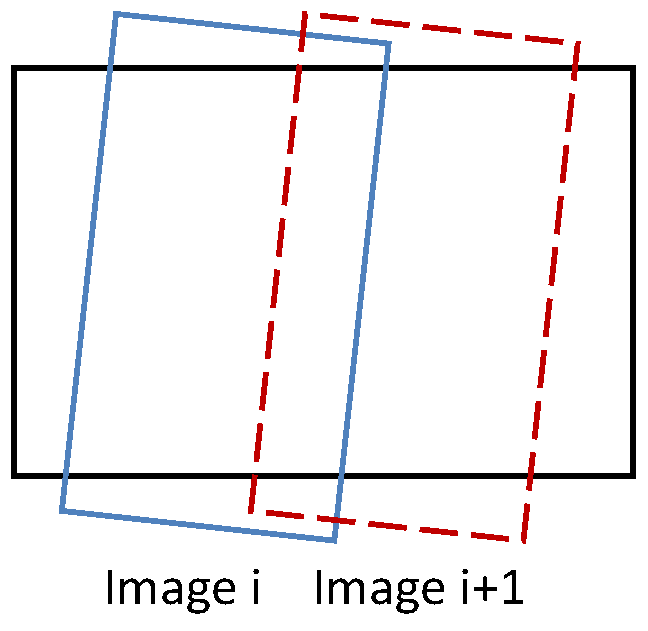
\includegraphics[width=1in]{projectionWall.pdf}}
  \centering
  \subfloat[][]{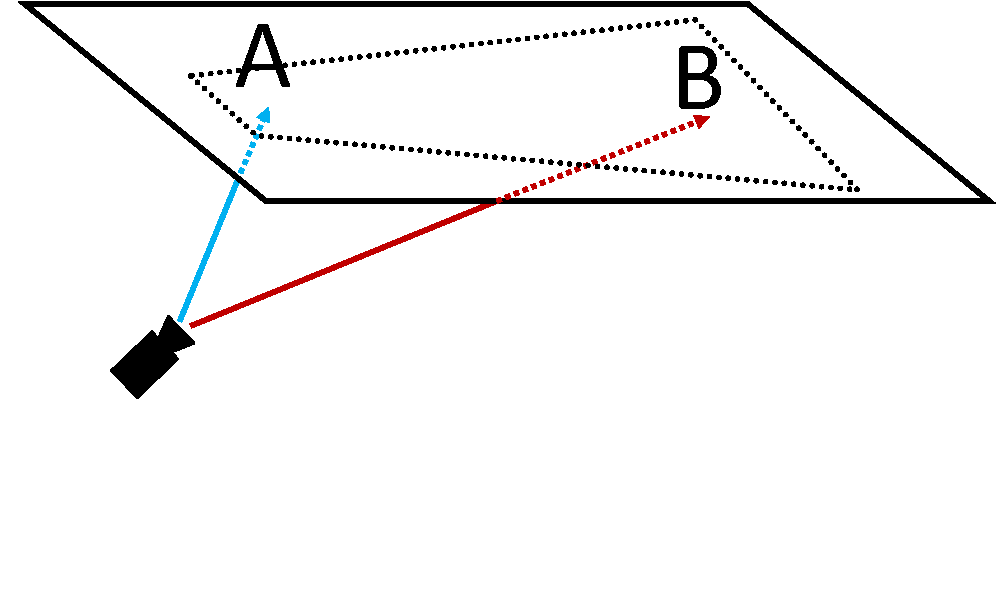
\includegraphics[width=1.1in]{projectionCeiling.pdf}}
  \centering
  \subfloat[][]{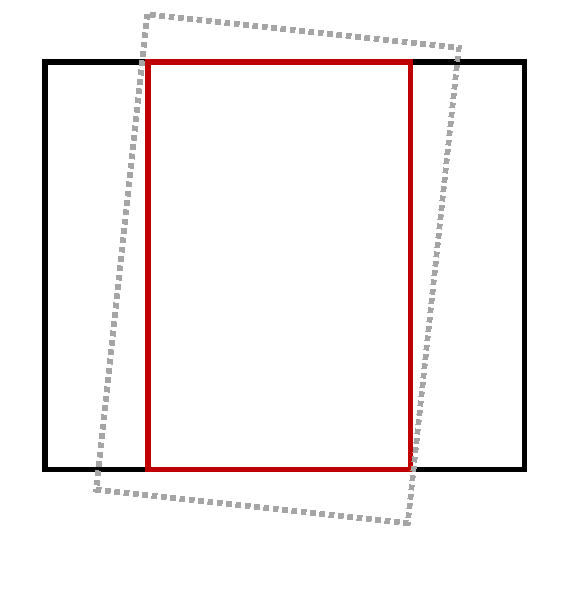
\includegraphics[width=0.9in]{projectionWallCrop.pdf}}
  \caption{(a) Undistorted fisheye images for vertical planes are
    tilted, but their effective camera axis is more or less normal to
    the plane. (b) The effective camera axis for ceilings is at an
    angle with respect to the plane normal. (c) Wall images are
    cropped to be rectangular.}
  \label{fig:projectionAngles}
\end{figure}



As mentioned earlier, the mobile backpack system used to capture data
in this paper contains 2 cameras with $180^\circ$ fisheye lenses
facing to the right and left. Since most human operators do not carry
the backpack in a perfectly upright position and are bent forwards at
15 to 20 degrees with respect to the vertical direction, the
undistorted fisheye images are head on with respect to vertical walls,
but at an angle with respect to horizontal floors and ceilings. This
is depicted for wall and ceiling planes in Figures
\ref{fig:projectionAngles}(a) and \ref{fig:projectionAngles}(b)
respectively. These oblique camera angles for ceilings translate into
textures that span extremely large areas once projected, as shown in
Figure \ref{fig:projectionAngles}(b). Using the tile-based texture
mapping criteria from Figure \ref{fig:scoringFunction}, such
projections have highly varying scores depending on the location on
the plane, as shown in Figure \ref{fig:projectionAngles}(b). Thus, the
tiling approach in Section \ref{sec:simpleTextureMapping} is a
reasonable choice for texturing floors and ceilings, as it uses the
parts of image projections that are viable choices for their
respective plane locations, e.g. areas near point A in Figure
\ref{fig:projectionAngles}(b), but not near point B.

\subsection{Tile-Mapping with Caching}
\label{sec:mappingWithCaching}
Since discontinuities occur where adjacent tiles select non-aligned
images, it makes sense to take into account image selections made by
neighboring tiles while texture mapping a given tile. By using the
same image across tile boundaries, we can eliminate a discontinuity
altogether. If this is not possible because a tile is not visible in
images used by neighboring tiles, using similar images across tile
boundaries also leads to less noticeable discontinuities.

Essentially a caching mechanism, we select the best image for a tile
$t$ by searching through two subsets of images for a viable candidate,
before searching through the entire set of valid images. The first
subset of images is the images selected by adjacent tiles that have
already been textured. We must first check which of these images can
map to $t$, and then of those, we make a choice according to the
scoring function in Figure \ref{fig:scoringFunction}. Before reusing
this image, we ensure it meets the criteria $\alpha < 45^\circ$, in
order to be considered a viable image, with $\alpha$ as the camera
angle as shown in Figure \ref{fig:scoringFunction}.

If no satisfactory image is found in the first subset, we check the
second subset of images, consisting of those taken near the ones in
the first subset, both spatially and temporally. These images are not
the same as the ones used for neighboring tiles, but are taken at a
similar location and time, suggesting that their localization and
projection are quite similar, allowing us to minimize any differences
in localization error as well as a parallax effects. Again, if no
viable image is found according to the same criteria, we search the
entire set of candidate images, selecting based on the same scoring
function from Figure \ref{fig:scoringFunction}.

The result of this caching approach is shown in Figure
\ref{fig:compareAll}(b). As compared to Figure
\ref{fig:compareAll}(a), discontinuities are reduced overall, but the
amount of remaining seams suggests that despite our high volume of
images, image selection alone cannot produce seamless textures. Camera
matrices, or the image projections themselves, have to be adjusted in
order to reliably generate clean textures.

\subsection{Shortest}
For wall planes however, most images are taken from close distances
and more or less head-on angles, resulting in higher resolution
fronto-parallel projections. As a result, for each tile on a wall
plane, the scoring function of Figure \ref{fig:scoringFunction} is
relatively flat with respect to a large number of captured images, as
they are all more or less head on. Thus, the scoring function is less
significant for walls, and it is conceivable to use a different
texturing strategy for them so as to minimize visible seams in texture
mapped planes. This can be done by choosing the smallest possible set
of images that (a) covers the entire plane and (b) minimizes the
amount of visible seams between them. A straightforward cost function
that accomplishes the latter is the Sum of Squared Differences (SSD)
of pixels in overlapping regions between all pairs of images, after
they have been rotated as described in Section
\ref{sec:projectionAndRotation}. Minimizing this cost function
encourages image boundaries to occur either in featureless areas, such
as bare walls, or in areas where images match extremely well.

To cover the entirety of a plane, our problem can be defined as
minimally covering a polygon i.e. the plane, using other polygons of
arbitrary geometry i.e. image projections, with the added constraint
of minimizing the cost function between chosen images.  This is a
complex problem, though we can take a number of steps to simplify it.

Given that wall-texture candidate images are taken from more or less
head-on angles, and assuming only minor rotations are made in Section
\ref{sec:projectionAndRotation}, we can reason that their projections
onto the plane are approximately rectangular. By cropping them all to
be rectangular, as shown in Figure \ref{fig:projectionAngles}(c), our
problem becomes the conceptually simpler one of filling a polygon with
rectangles, such that the sum of all costs between each pair of
rectangles is minimal. We thus also retain the advantages of working
with rectangular units, as explained in Section
\ref{sec:simpleTextureMapping}.

The location and orientation of the cameras and the fisheye lenses on
the acquisition backpack is such that images nearly always contain the
entirety of the floor to ceiling range of wall planes. Images are
therefore rarely projected with one above another when texturing wall
planes. In essence, we need only to ensure lateral coverage of wall
planes, e.g. from left to right, as our images provide full vertical
coverage themselves. We can thus construct a Directed Acyclic Graph
(DAG) from the images, with edge costs defined by the SSD cost
function, and solve a simple shortest path problem to find an optimal
subset of images with regard to the cost function \cite{dijkstra}.

\begin{figure}
  \centering
  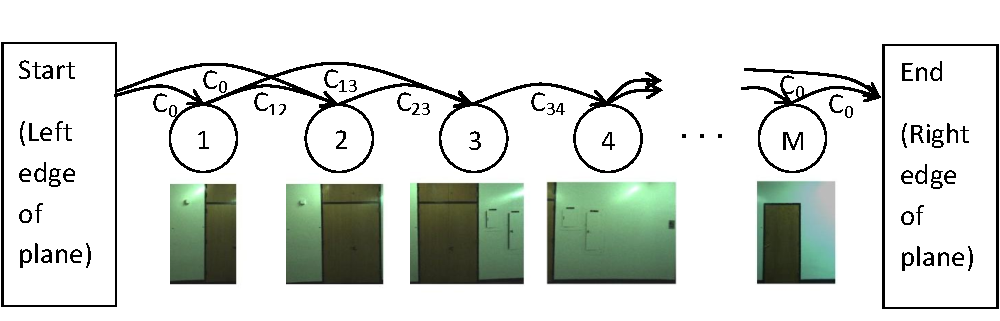
\includegraphics[width=3in]{dagCreation.pdf}
  \caption{DAG construction for the image selection process. \\}
  \label{fig:dagCreation}
\end{figure}

Figure \ref{fig:dagCreation} demonstrates the construction of a DAG
from overlapping images of a long hallway. Images are sorted by
horizontal location left to right, and become nodes in a
graph. Directed edges are placed in the graph from left to right
between overlapping images. The weights of these edges are determined
by the SSD cost function. Next, we add two artificial nodes, one start
node representing the left border of the plane, and one end node
representing the right border of the plane. The left(right) artificial
node has directed edges with equal cost $C_0$ to(from) all images that
meet the left(right) border of the plane.

We now solve the shortest path problem from the start node to the end
node. This results in a set of images completely covering the plane
horizontally, while minimizing the cost of seams between images.

In rare cases where the vertical dimension of the plane is not
entirely covered by one or more chosen images, we are left with holes
where no images are selected to texture. To address this, we solve for
a new shortest path after modifying the edges chosen by the original
shortest path solution such that they have higher cost than all other
edges in the DAG, and solve for a new shortest path. This ensures that
these edges are not chosen again unless they are the only available
option. Our second shortest path solution results in a new set of
chosen images, of which we only retain those that cover areas not
covered by the first set. This process can be repeated as many times
as needed, until holes are no longer present. This method is not as
optimal as a 2D-coverage solution would be, but it is a fast
approximation, and adequately handles the few holes we encounter.

With this completed, we have now mapped every location on the plane to
at least one image, and have minimized the number of images, as well
as the discontinuities between their borders. As seen in Figure
\ref{fig:compareAll}(d), this seam minimization method has fewer
visible discontinuities than Figure \ref{fig:compareAll}(c)
corresponding to the tile caching approach\footnote{In Figure
  \ref{fig:compareAll}(d), we arbitrarily chose one image for
  texturing where images overlap, as blending will be discussed in the
  next section.}. This is especially evident when comparing the
posters in the images, which have clear misalignment over seams in
Figure \ref{fig:compareAll}(c), but are much more aligned in Figure
\ref{fig:compareAll}(d). This is because the seam minimization
approach directly reduces the cost of each image boundary, while the
tile caching method uses a scoring function that only approximates
this effect. Furthermore, seam minimization guarantees the best
selection of images, while the sequential tile caching method may
select images early on that turn out to be poor choices once
subsequent tiles have been processed. The seam minimization approach
is also far less intensive in terms of memory usage and runtime, both
during texture generation and rendering, as it does not require
discretizing planes or images\footnote {For the seam minimization
  approach, occlusion checks are performed over the entirety of each
  image to determine available areas for texture mapping. Since indoor
  environments mostly consist of vertical or horizontal surfaces with
  high amounts of right angles, image projections remain largely
  rectangular after masking out occluded areas. Therefore, as a
  preprocessing step, we can recursively split each image into
  rectangular pieces and check for occlusions in a similar manner as
  in the tiling process.  }.

In the context of texturing an entire 3D planar model, we choose to
apply the seam minimization approach on walls, due to its superior
output when provided with head-on images. Floors and ceilings however,
given their many images taken at oblique angles, are textured using
the tile caching method.

% \begin{figure*}
%   \centering
%   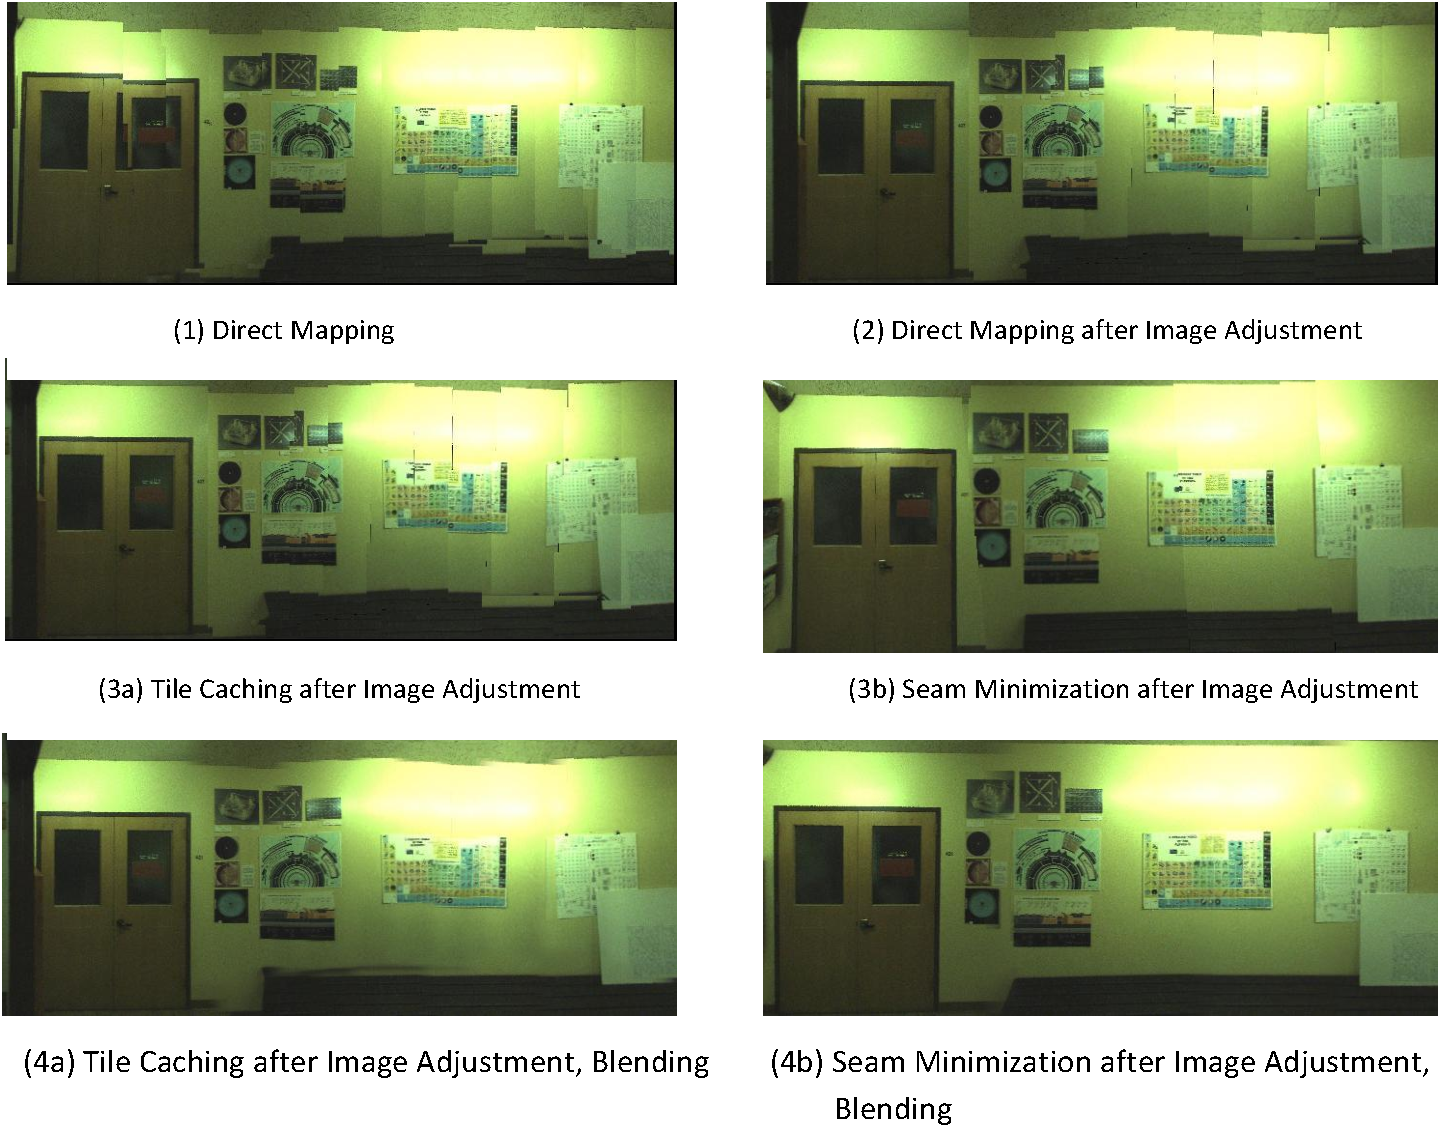
\includegraphics[width=6in]{pipelineimages.pdf}
%   \caption{Textures corresponding to each step in our texture
%   mapping pipeline.}
%   \label{fig:pipelineimages}
% \end{figure*}


\subsection{Blending}
\label{sec:blending}
We now apply the same blending process to the two texturing methods:
image alignment followed by either tile caching or seam minimization.

Although the preprocessing steps and image selection in both methods
attempt to minimize all mismatches between images, there are
occasional unavoidable discontinuities in the final texture due to
different lighting conditions or inaccuracies in planar geometry or
projection. These can however be treated and smoothed over by applying
alpha blending over image seams.  Whether the units we are blending
are rectangularly-cropped images or rectangular tiles, we can apply
the same blending procedure, as long as we have a guaranteed overlap
between units to blend over.

For the tile caching method, we can ensure overlap by texturing a
larger tile than needed for display. For example, for a rendered tile
$l_1 \times l_1$, we can associate it with a texture $(l_1 + l_2)
\times (l_1 + l_2)$ in size. For the seam minimization method, we have
already ensured overlap between images. To enforce consistent blending
however, we add a minimum required overlap distance while solving the
shortest path problem in Section
\ref{sec:seamMinimization}. Additionally, if images overlap in a
region greater than the overlap distance, we only apply blending over
an area equal to the overlap distance.

After blending pixels linearly across overlapping regions using alpha
blending, texture mapping is complete. Figures \ref{fig:compareAll}(e)
and \ref{fig:compareAll}(f) show the blended versions of Figures
\ref{fig:compareAll}(c) and \ref{fig:compareAll}(d) respectively. It
is clear that the seam minimization approach still exhibits better
alignment and fewer seams than the tile-caching method, as Figure
\ref{fig:compareAll}(f) has the best visual quality among the textures
in Figure \ref{fig:compareAll}.

\section{Results and Conclusions}
\label{sec:resultsAndConclusions}


%%%%%%%%%%%%%%%%%%%%%%%%%%%%%%%%%%%%%%%%%%%%%%%%%%%%%%%%%%%%%
%%%%% References %%%%%

\bibliography{report} %>>>> bibliography data in report.bib
\bibliographystyle{spiebib} %>>>> makes bibtex use spiebib.bst

\end{document} 
